%%%%%%%%%%%%%%%%%%%%%%%%%%%%%%%%%%%%%%%%%%%%%%%%%%%%%%%%%%%%%%%%%%%%%%%%%%%%%%%%
%%%%%%%%%%%%%%%%%%%%%%%%%%%%%%%%%%%%%%%%%%%%%%%%%%%%%%%%%%%%%%%%%%%%%%%%%%%%%%%%
%%%%%%%%%%%%%%%%%%%%%%%%%%%%%%%%%%%%%%%%%%%%%%%%%%%%%%%%%%%%%%%%%%%%%%%%%%%%%%%%
%%%%%%%%%%%%%%%%%%%%%%%%%%%%%%%%%%%%%%%%%%%%%%%%%%%%%%%%%%%%%%%%%%%%%%%%%%%%%%%%
\chapter{Performances des systèmes asservis\label{chap-perf}}
%%%%%%%%%%%%%%%%%%%%%%%%%%%%%%%%%%%%%%%%%%%%%%%%%%%%%%%%%%%%%%%%%%%%%%%%%%%%%%%%
%%%%%%%%%%%%%%%%%%%%%%%%%%%%%%%%%%%%%%%%%%%%%%%%%%%%%%%%%%%%%%%%%%%%%%%%%%%%%%%%
%%%%%%%%%%%%%%%%%%%%%%%%%%%%%%%%%%%%%%%%%%%%%%%%%%%%%%%%%%%%%%%%%%%%%%%%%%%%%%%%
%%%%%%%%%%%%%%%%%%%%%%%%%%%%%%%%%%%%%%%%%%%%%%%%%%%%%%%%%%%%%%%%%%%%%%%%%%%%%%%%

\minitoc
\newpage

%%%%%%%%%%%%%%%%%%%%%%%%%%%%%%%%%%%%%%%%%%%%%%%%%%%%%%%%%%%%%%%%%%%%%%%%%%%%%%%%
%%%%%%%%%%%%%%%%%%%%%%%%%%%%%%%%%%%%%%%%%%%%%%%%%%%%%%%%%%%%%%%%%%%%%%%%%%%%%%%%
%%%%%%%%%%%%%%%%%%%%%%%%%%%%%%%%%%%%%%%%%%%%%%%%%%%%%%%%%%%%%%%%%%%%%%%%%%%%%%%%
\section{Introduction}
%%%%%%%%%%%%%%%%%%%%%%%%%%%%%%%%%%%%%%%%%%%%%%%%%%%%%%%%%%%%%%%%%%%%%%%%%%%%%%%%
%%%%%%%%%%%%%%%%%%%%%%%%%%%%%%%%%%%%%%%%%%%%%%%%%%%%%%%%%%%%%%%%%%%%%%%%%%%%%%%%
%%%%%%%%%%%%%%%%%%%%%%%%%%%%%%%%%%%%%%%%%%%%%%%%%%%%%%%%%%%%%%%%%%%%%%%%%%%%%%%%
Les performances qui vont nous interesser dans 
ce chapitre sont la \textbf{précision} et la \textbf{rapidité}.
Dans les deux cas, nous allons observer que les performances
en boucle fermée dépendent du système en boucle ouverte. 

%%%%%%%%%%%%%%%%%%%%%%%%%%%%%%%%%%%%%%%%%%%%%%%%%%%%%%%%%%%%%%%%%%%%%%%%%%%%%%%%
%%%%%%%%%%%%%%%%%%%%%%%%%%%%%%%%%%%%%%%%%%%%%%%%%%%%%%%%%%%%%%%%%%%%%%%%%%%%%%%%
%%%%%%%%%%%%%%%%%%%%%%%%%%%%%%%%%%%%%%%%%%%%%%%%%%%%%%%%%%%%%%%%%%%%%%%%%%%%%%%%
\section{Précision}
%%%%%%%%%%%%%%%%%%%%%%%%%%%%%%%%%%%%%%%%%%%%%%%%%%%%%%%%%%%%%%%%%%%%%%%%%%%%%%%%
%%%%%%%%%%%%%%%%%%%%%%%%%%%%%%%%%%%%%%%%%%%%%%%%%%%%%%%%%%%%%%%%%%%%%%%%%%%%%%%%
%%%%%%%%%%%%%%%%%%%%%%%%%%%%%%%%%%%%%%%%%%%%%%%%%%%%%%%%%%%%%%%%%%%%%%%%%%%%%%%%
Un système est précis si l'écart que l'on note $\epsilon(t)$ 
entre l'entrée $e(t)$ et la sortie $s(t)$ est nul.
Dans le domaine de Laplace, cet écart devient :
$$
\epsilon(p)=E(p)-S(p)
$$

On distingue deux cas :
\begin{itemize}
    \item En régime permanent, cet écart $\epsilon_s$ est nommée 
		  \textbf{erreur statique. }
    \item En régime transitoire, cet écart $\epsilon(t)=e(t)-s(t)$ est 
		  nommée \textbf{erreur dynamique.}
\end{itemize}

L'erreur dynamique consiste à suivre l'écart défini précedemment durant 
le transitoire.

Pour étudier l'erreur statique, on sollicite le système à différents 
types de signaux pour obtenir dans les différents cas :
\begin{itemize}
	\item l'\textbf{erreur indicielle} ou l'erreur de position qui est 
		  l'erreur statique de la réponse indicielle.
	\item l'\textbf{erreur de poursuite} ou erreur de vitesse qui est 
		  l'erreur statique de la réponse à une rampe.
	\item l'\textbf{erreur en accélération} qui est l'erreur statique 
		  de la réponse à une parabole.
\end{itemize}
Concrétement pour étudier l'erreur statique on cherche la limite à l'infini 
de $\epsilon(t)$ ou encore en appliquant le théorème de la valeur finale :
\begin{bequation}[ams align]
\epsilon(\infty)=\lim\limits_{t\to\infty} e(t)-s(t)
	            =\lim\limits_{p\to 0} p\big(E(p)-S(p)\big)
\end{bequation}
Rappelons que pour pouvoir appliquer ce théorème la valeur finale doit 
être finie ou en d'autre mot le système doit être stable.

%%%%%%%%%%%%%%%%%%%%%%%%%%%%%%%%%%%%%%%%%%%%%%%%%%%%%%%%%%%%%%%%%%%%%%%%%%%%%%%%
%%%%%%%%%%%%%%%%%%%%%%%%%%%%%%%%%%%%%%%%%%%%%%%%%%%%%%%%%%%%%%%%%%%%%%%%%%%%%%%%
\subsection{Précision en boucle ouverte}
%%%%%%%%%%%%%%%%%%%%%%%%%%%%%%%%%%%%%%%%%%%%%%%%%%%%%%%%%%%%%%%%%%%%%%%%%%%%%%%%
%%%%%%%%%%%%%%%%%%%%%%%%%%%%%%%%%%%%%%%%%%%%%%%%%%%%%%%%%%%%%%%%%%%%%%%%%%%%%%%%

Soit un système caractérisé par la fonction de transfert $H(p)$ 
est sollicité par l'entrée $E(p)$. La sortie $S(p)$ est alors donnée par :

\begin{center}
\tikzsetnextfilename{sb_bloc1-chap6-ext}
\begin{tikzpicture}
    \sbEntree{E}
    \sbBloc[3]{H}{$H(p)$}{E}
    \sbRelier[$E(p)$]{E}{H}
    \sbSortie[3]{S}{H}
    \sbRelier[$S(p)$]{H}{S}
\end{tikzpicture}
\end{center}

L'erreur statique est alors donnée par :
$$
\epsilon(\infty)=\lim\limits_{p\to 0} p\big(E(p)-H(p)E(p)\big)
                =\lim\limits_{p\to 0} p\big(1-H(p)\big)E(p)
$$
%%%%%%%%%%%%%%%%%%%%%%%%%%%%%%%%%%%%%%%%%%%%%%%%%%%%%%%%%%%%%%%%%%%%%%%%%%%%%%%%
\subsubsection{Exemple d'un premier ordre}
%%%%%%%%%%%%%%%%%%%%%%%%%%%%%%%%%%%%%%%%%%%%%%%%%%%%%%%%%%%%%%%%%%%%%%%%%%%%%%%%
%Rappelons qu'il est possible de corriger la précision 
%d'un système en boucle ouverte. 
Prenons l'exemple d'un système du 1er ordre de fonction de transfert canonique 
$H(p)=\dfrac{K}{1+\tau p}$ que l'on sollicite avec un échelon 
d'amplitude (consigne) $E_0$.
L'erreur statique est alors donnée par :
$$
\epsilon(\infty)=\lim\limits_{p\to 0}\left(1-\dfrac{K}{1+\tau p}\right)E_0
                =(1-K)E_0
$$

Le système est prècis (c.a.d $\epsilon(\infty)=0$) si $K=1$. 

%Il alors possible de corriger en boucle ouverte la précision en 
%introduisant un gain $K'$ :

%\begin{center}
%\tikzsetnextfilename{sb_bloc2-chap6-ext}
%\begin{tikzpicture}
%    \sbEntree{E}
%	\sbBloc[3]{C}{$K'$}{E}
%    \sbRelier[$E(p)$]{E}{C}
%	\sbBloc[3]{H}{$\dfrac{K}{1+\tau p}$}{C}
%    \sbRelier[$U(p)$]{C}{H}
%    \sbSortie[3]{S}{H}
%    \sbRelier[$S(p)$]{H}{S}
%\end{tikzpicture}
%\end{center}
%tel que $K'K=1$ ou encore $K'=\frac{1}{K}$.

%Cependant, nous allons dans ce chapitre nous interesser uniquement 
% à l'asservissement en %boucle fermée.

%%%%%%%%%%%%%%%%%%%%%%%%%%%%%%%%%%%%%%%%%%%%%%%%%%%%%%%%%%%%%%%%%%%%%%%%%%%%%%%%
%%%%%%%%%%%%%%%%%%%%%%%%%%%%%%%%%%%%%%%%%%%%%%%%%%%%%%%%%%%%%%%%%%%%%%%%%%%%%%%%
\subsection{Précision en boucle fermée}
%%%%%%%%%%%%%%%%%%%%%%%%%%%%%%%%%%%%%%%%%%%%%%%%%%%%%%%%%%%%%%%%%%%%%%%%%%%%%%%%
%%%%%%%%%%%%%%%%%%%%%%%%%%%%%%%%%%%%%%%%%%%%%%%%%%%%%%%%%%%%%%%%%%%%%%%%%%%%%%%%

Considérons le cas d'un système asservi de fonction de transfert $H(p)$
par une boucle de contre-réaction à retour unitaire.

\begin{center}
\tikzsetnextfilename{sb_bloc3-chap6-ext}
\begin{tikzpicture}
    \sbEntree{E}
    \sbComp{comp1}{E}
    \sbRelier[$E(p)$]{E}{comp1}
    \sbBloc[3]{H}{$H(p)$}{comp1}
    \sbRelier[$\epsilon(p)$]{comp1}{H}
    \sbSortie[3]{S}{H}
    \sbRelier[$S(p)$]{H}{S}
    \sbRenvoi[4]{H-S}{comp1}{}
\end{tikzpicture}
\end{center}

La~\gls{ftbo} est simplement donnée par $H(p)$. Dans le cas le plus
générale, il est toujours possible d'écrire une fonction de transfert
sous la forme canonique (\Cref{chap-slci}) :
$$
H_{BO}(p)=\dfrac{K}{p^\alpha}\cdot\dfrac{N(p)}{D(p)}
$$
avec $\alpha$ la classe du système en boucle ouverte, $K$ le gain statique et 
$N(p)$ et $D(p)$ deux polynômes tels que $N(0)=D(0)=1$. 


Dans le domaine de Laplace l'écart $\epsilon(p)$ s'écrit :
$$
\epsilon(p)=E(p)-S(p)=\left(1-\dfrac{H_{BO}(p)}{1+H_{BO}(p)}\right)E(p)
$$
en remplaçant $H_{BO}(p)$ par sa représentation générale:
\begin{bequation}[ams align]
\epsilon(p)=\dfrac{p^\alpha D(p)}{p^\alpha D(p)+KN(p)}E(p)
\end{bequation}

L'erreur statique $\epsilon_s$ est alors donnée par la limite (Théorème 
de la valeur finale) :
$$
\epsilon_s=\lim\limits_{p\to 0} p\epsilon(p)=\lim\limits_{p\to 0} 
           \dfrac{p^\alpha D(p)}{p^\alpha D(p)+KN(p)}pE(p) 
$$
ou encore en utilisant les valeurs des polynômes en 0: 
\begin{bequation}[ams align]
	\epsilon_s=\lim\limits_{p\to 0} \dfrac{p^\alpha}{p^\alpha+K}pE(p)
	\label{eq-erreurStatique}
\end{bequation}

Cette erreur dépend donc de la nature de la sollicitation (c.a.d $E(p)$) et 
de la classe $\alpha$ de la fonction de transfert en boucle ouverte.

Nous allons maintenant considérer différentes types de sollicitations pour 
différentes classes de système en boucle ouverte.

%%%%%%%%%%%%%%%%%%%%%%%%%%%%%%%%%%%%%%%%%%%%%%%%%%%%%%%%%%%%%%%%%%%%%%%%%%%%%%%%
\subsubsection{Erreur statique indicielle}
%%%%%%%%%%%%%%%%%%%%%%%%%%%%%%%%%%%%%%%%%%%%%%%%%%%%%%%%%%%%%%%%%%%%%%%%%%%%%%%%

L'erreur indicielle est l'erreur entre la sortie d'un système et une 
sollicitation en échelon $e(t)=E_0u(t)$ de transformée de Laplace 
$E(p)=\dfrac{E_0}{p}$. 
Pour une telle entrée, l'erreur statique (c.f \cref{eq-erreurStatique}) 
devient :
$$
\epsilon_s=\lim\limits_{p\to 0} \dfrac{p^\alpha}{p^\alpha+K}E_0
$$

Dans le cas d'un système de classe $\alpha=0$ en boucle ouverte :
$$
\epsilon_s=\lim\limits_{p\to 0} \dfrac{p^0}{p^0+K}E_0=\dfrac{E_0}{1+K}.
$$
L'erreur est finie mais les réponses indicielles des systèmes de classe 
$\alpha=0$ en boucle ouverte ne sont pas précis.

Dans les autres cas $\alpha>0$, l'erreur statique s'annule :
$$
\epsilon_s=\lim\limits_{p\to 0} \dfrac{p^\alpha}{p^\alpha+K}E_0=0
$$
Les réponses indicielle des systèmes de classe $\alpha>0$ sont donc précis.

%%%%%%%%%%%%%%%%%%%%%%%%%%%%%%%%%%%%%%%%%%%%%%%%%%%%%%%%%%%%%%%%%%%%%%%%%%%%%%%%
\subsubsection{Erreur statique de poursuite}
%%%%%%%%%%%%%%%%%%%%%%%%%%%%%%%%%%%%%%%%%%%%%%%%%%%%%%%%%%%%%%%%%%%%%%%%%%%%%%%%
L'erreur de poursuite est l'erreur statique d'un système soumis à une rampe 
du type $e(t)=r(t)=E_0t u(t)$
de transformée de Laplace $E(p)=\dfrac{E_0}{p^2}$

Pour une telle entrée, l'erreur statique devient :
$$
\epsilon_s=\lim\limits_{p\to 0} \dfrac{p^\alpha}{p^\alpha+K}\dfrac{E_0}{p}
          =\dfrac{p^{\alpha-1}}{p^\alpha+K}E_0 
$$

Dans le cas d'un système de classe $\alpha=0$ en boucle ouverte, 
l'erreur devient :
$$
\epsilon_s=\lim\limits_{p\to 0}\dfrac{p^{-1}}{p^0+K}E_0=+\infty
$$
Le système est incapable de suivre l'entrée souhaitée.

Dans le cas d'un système de classe $\alpha=1$ en boucle ouverte, 
l'erreur devient :
$$
\epsilon_s=\lim\limits_{p\to 0}\dfrac{p^0}{p+K}E_0=\dfrac{E_0}{K}
$$

Dans le cas d'un système de classe $\alpha>1$ en boucle ouverte, 
l'erreur devient :
$$
\epsilon_s=\lim\limits_{p\to 0}\dfrac{p^{\alpha-1}}{p^\alpha+K}E_0=0
$$
Le système est donc prècis.

%%%%%%%%%%%%%%%%%%%%%%%%%%%%%%%%%%%%%%%%%%%%%%%%%%%%%%%%%%%%%%%%%%%%%%%%%%%%%%%%
\subsubsection{Erreur statique d'accélération}
%%%%%%%%%%%%%%%%%%%%%%%%%%%%%%%%%%%%%%%%%%%%%%%%%%%%%%%%%%%%%%%%%%%%%%%%%%%%%%%%

L'erreur d'accélération est l'erreur statique d'un système soumis à un signal
parabolique $e(t)=E_0t^2 u(t)$ de transformée de Laplace 
$E(p)=\dfrac{2E_0}{p^3}$

Pour une telle entrée, l'erreur statique devient :
$$
\epsilon_s=\lim\limits_{p\to 0} \dfrac{p^\alpha}{p^\alpha+K}\dfrac{2E_0}{p^2}
          =\dfrac{p^{\alpha-2}}{p^\alpha+K}2E_0 
$$

Dans le cas d'un système de classe $\alpha<2$ en boucle ouverte, 
l'erreur devient :
$$
\epsilon_s=+\infty
$$

Pour un système de classe $\alpha=2$ en boucle ouverte, 
l'erreur est finie :
$$
\epsilon_s=\dfrac{2E_0}{K}
$$
et s'annule pour $\alpha>2$

\begin{table}
    \ra{2.0}
    \centering
    \begin{tabular}{@{}P{2cm}P{2cm}P{2cm}P{2cm}P{2cm}@{}}
    \toprule
    Entrée & $\alpha=0$ & $\alpha=1$ & $\alpha=2$ & $\alpha>2$ \\
    \midrule
    $\dfrac{E_0}{p}$&$\dfrac{E_0}{1+K}$&0&0&0\\
    $\dfrac{E_0}{p^2}$&$+\infty$&$\dfrac{E_0}{K}$&0&0\\
    $\dfrac{2E_0}{p^3}$&$+\infty$&$+\infty$&$\dfrac{2E_0}{K}$&0\\
    \bottomrule
    \end{tabular}
\caption{Résumé des erreurs statiques pour différentes 
         sollicitations et classe de système en boucle ouverte}
\end{table}

%%%%%%%%%%%%%%%%%%%%%%%%%%%%%%%%%%%%%%%%%%%%%%%%%%%%%%%%%%%%%%%%%%%%%%%%%%%%%%%%
%%%%%%%%%%%%%%%%%%%%%%%%%%%%%%%%%%%%%%%%%%%%%%%%%%%%%%%%%%%%%%%%%%%%%%%%%%%%%%%%
\subsection{Effet d'une perturbation}
%%%%%%%%%%%%%%%%%%%%%%%%%%%%%%%%%%%%%%%%%%%%%%%%%%%%%%%%%%%%%%%%%%%%%%%%%%%%%%%%
%%%%%%%%%%%%%%%%%%%%%%%%%%%%%%%%%%%%%%%%%%%%%%%%%%%%%%%%%%%%%%%%%%%%%%%%%%%%%%%%

%%%%%%%%%%%%%%%%%%%%%%%%%%%%%%%%%%%%%%%%%%%%%%%%%%%%%%%%%%%%%%%%%%%%%%%%%%%%%%%%
\subsubsection{Cas générale}
%%%%%%%%%%%%%%%%%%%%%%%%%%%%%%%%%%%%%%%%%%%%%%%%%%%%%%%%%%%%%%%%%%%%%%%%%%%%%%%%

On considère maintenant l'effet d'une perturbation sur la précision d'un 
système asservis. 

Sans perte de généralité, on considère une perturbation 
en entrée (c'est à dire en amont d'un système linéaire défini par une fonction 
de transfert $H_2(p)$, la présence d'un correcteur $H_1(p)$ n'est pas 
obligatoire mais facilite l'interprétation des résultats. 

Soit le schéma-bloc suivant, présentant un système asservi par la consigne 
$E(p)$ et soumis à une perturbation $P(p)$.

\begin{center}
\tikzsetnextfilename{reduc_mult1-chap6-ext}
\begin{tikzpicture}
    \cpbruni[$E(p)$]
        [$\epsilon(p)$]
        [$H_1(p)$]
        [ ]
        [ ]
        [$P(p)$]
        [$H_2(p)$]
        []
        [$S(p)$]
\end{tikzpicture}
\end{center}

On se donne les formes canoniques suivantes pour les deux fonctions de 
transferts $H_1(p)$ et $H_2(p)$ tels que :
\begin{align*}
H_1(p)=\dfrac{K_1}{p^{\alpha_1}}\dfrac{N_1(p)}{D_1(p)}\\
H_2(p)=\dfrac{K_2}{p^{\alpha_2}}\dfrac{N_2(p)}{D_2(p)}
\end{align*}
avec $K_i$, $\alpha_i$, $N_i(p)$ et $D_i(p)$ respectivement les gains statiques,
la classe et les polynômes en $p$ tels que $N_i(0)=1$ et $D_i(0)=1$.

Pour déterminer l'écart, il nous faut déterminer la sortie globale $S(p)$ pour
des entrées multiples (c.f~\Cref{chap-schemabloc}-\cref{sec-multE}).
Cette sortie est sous la forme :
$$
S(p)=H_{P=0}E(p)+H_{E=0}P(p)
$$
c'est à dire que c'est la somme des contributions des deux entrées prises
séparemment.
L'écart est alors donné par 
$$
\epsilon(p)=E(p)-S(p)=\left(1-H_{P=0}\right)E(p)-H_{E=0}P(p)
$$
Le premier terme correspond à l'écart de l'asservissement que nous avons 
déjà étudié précedemment, le second terme, que l'on note $\epsilon_P(p)$, 
est la contribution à l'écart dû à la perturbation.
La fonction de transfert de l'asservissement est donnée par :
$$
H_{P=0}=\dfrac{H_1H_2(p)}{1+H_1(p)H_2(p)} 
$$

Dans le cas de la régulation d'un système asservis, il est nécessaire de 
rejeter cette contribution.

La fonction de transfert $H_{E=0}$, de la régulation, correspondant à une 
consigne nulle, s'obtient en considérant le schéma-bloc suivant :

\begin{center}                                                  
\tikzsetnextfilename{pert1-chap6-ext}
    \begin{tikzpicture}                                         
        \bbr[$P(p)$][][$H_2(p)$][][$S(p)$][$H_1(p)$][][ ] 
    \end{tikzpicture}                                           
\end{center}                                                    

\newcommand{\pau}{p^{\alpha_1}}
\newcommand{\pad}{p^{\alpha_2}}
en boucle fermée, on a alors:
$$
H_{E=0}(p)=\dfrac{H_2(p)}{1+H_1(p)H_2(p)}
$$
en remplaçant par leurs formes canoniques générales :
$$
H_{E=0}(p)=
\dfrac{\pau K_2N_2(p)D_1(p)}{\pau\pad D_1(p)D_2(p)+K_1K_2N_1(p)N_2(p)}
$$

Examinons l'erreur en régime permanent pour une perturbation constante.
C'est à dire pour perturbation $P(p)$ en échelon telle que 
$P(p)=\dfrac{P_0}{p}$. L'erreur dû à la perturbation en régime permanent 
est alors :
\begin{align*}
\epsilon_P&=\lim\limits_{p\to0} p\epsilon_P\\
\epsilon_P&=\lim\limits_{p\to0} -H_{E=0}P_0\\
\epsilon_P&=\lim\limits_{p\to0}\dfrac{\pau K_2}{\pau\pad+K_1K_2}P_0
\end{align*}
\textbf{La perturbation est rejétée si $\alpha_1>0$, c'est à dire s'il existe
au moins un intégrateur en amont de la perturbation.}
En effet si $\alpha_1=0$, l'erreur dû à la perturbation est finie et 
donnée par :
$$
\epsilon_P=\lim\limits_{p\to0}\dfrac{K_2}{\pau\pad+K_1K_2}P_0
$$

%%%%%%%%%%%%%%%%%%%%%%%%%%%%%%%%%%%%%%%%%%%%%%%%%%%%%%%%%%%%%%%%%%%%%%%%%%%%%%%%
\subsubsection{Exemple de rejet de perturbation}
%%%%%%%%%%%%%%%%%%%%%%%%%%%%%%%%%%%%%%%%%%%%%%%%%%%%%%%%%%%%%%%%%%%%%%%%%%%%%%%%
Nous allons voir ici le rejet d'une perturbation d'un système du premier ordre. 
On considère le système du premier ordre, en boucle ouverte, placé dans une 
boucle de contre réaction unitaire avec un intégrateur comme ci-dessous :
\begin{center}                           
\tikzsetnextfilename{pert2-chap6-ext}
    \begin{tikzpicture}                  
    \sbEntree{E}
    \sbComp{comp1}{E}
    \sbRelier[$E(p)$]{E}{comp1}
    \sbBloc[3]{C}{$\dfrac{1}{p}$}{comp1}
    \sbRelier[$\epsilon(p)$]{comp1}{C}
    \sbBloc[3]{H}{$\dfrac{1}{p+1}$}{C}
    \sbRelier[]{C}{H}
    \sbSortie[3]{S}{H}
    \sbRelier[$S(p)$]{H}{S}
    \sbRenvoi[4]{H-S}{comp1}{}
    \end{tikzpicture}                    
\end{center}                             
On souhaite réguler ce système pour une consigne en échelon.
D'après les résultats précédents, l'erreur statique de position est nulle 
en asservissement puisque le système présente au moins un intégrateur. 
Pour observer le rejet de la perturbation, nous allons considérer 
deux positions possibles pour la perturbation (avant et après 
l'intégrateur). On considère une perturbation constante telle 
que $P(p)=e^{-\tau p}\dfrac{P_0}{p}$ retardée d'un temps $\tau>0$. 
%%%%%%%%%%%%%%%%%%%%%%%%%%%%%%%%%%%%%%%%%%%%%%%%%%%%%%%%%%%%%%%%%%%%%%%%%%%%%%%%
\paragraph{Si l'intégrateur est en aval de la perturbation}
%%%%%%%%%%%%%%%%%%%%%%%%%%%%%%%%%%%%%%%%%%%%%%%%%%%%%%%%%%%%%%%%%%%%%%%%%%%%%%%%
Dans un tel cas l'erreur dû à la perturbation est donnée par :
$$
\epsilon_P=\lim\limits_{p\to0}p\epsilon_P(p)=
\lim\limits_{p\to0}\dfrac{e^{-\tau p}}{p(p+1)+1}P_0=P_0
$$
L'erreur statique de position totale est donc non nulle. La perturbation
n'est pas rejétée comme on peut le voir sur la simulation de la réponse
temporelle globale de ce système (c.f~\cref{fig-pert1}).
\begin{figure}[!h]
\centering
\tikzsetnextfilename{pert1_data-chap6-ext}
\begin{tikzpicture}
    \begin{axis}
    [   legend style={draw=none,font=\normalsize},
        legend pos=outer north east,
        axis line style = thick,
        width=0.45\textwidth,
        xmin=0,
        xmax=30,
        ymin=0,
        ymax=1.75,
        xlabel={$t$},
        ylabel={$s(t)$},
        label style={font=\Large},
        legend cell align={left},
    ]%
        \addplot[mark=none,vtb] table {scilab/pert1_data.tab};
        \addplot[red,thick,domain=0:15] {1};   %échelon
        \addplot[red,thick,domain=15:30] {1.5}; %pertubation
        \addplot[red,thick,domain=-2:0] {0};
        \draw[red,thick,dashed] (0,0)--(0,1);   %échelon
        \draw[red,thick,dashed] (15,1)--(15,1.5);   %échelon
    \end{axis}
    \begin{scope}[shift={(-10,2.3)}]
        \sbEntree{E}
        \sbCompSum{comp1}{E}{+}{-}{+}{}
        \sbRelier[$E(p)$]{E}{comp1}
        \sbBloc[2.5]{C}{$\dfrac{1}{p}$}{comp1}
        \sbRelier[$\epsilon(p)$]{comp1}{C}
        \sbBloc[3]{H}{$\dfrac{1}{p+1}$}{C}
        \sbRelier[]{C}{H}
        \sbSortie[3]{S}{H}
        \sbRelier[$S(p)$]{H}{S}
        \sbRenvoi[4]{H-S}{comp1}{}
        \sbDecaleNoeudy[-2.5]{comp1}{P}
        \sbRenvoiF[-2.5]{P}{comp1}{$P(p)$}
    \end{scope}
\end{tikzpicture}
\caption{Effet de la perturbation sur la réponse temporelle dans le cas
         où l'intégrateur est en aval de la perturbation. La simulation 
         de la réponse temporelle est obtenue pour les paramètres suivants:
         $E_0=1$, $\tau=15$\label{fig-pert1}}
\end{figure}
%%%%%%%%%%%%%%%%%%%%%%%%%%%%%%%%%%%%%%%%%%%%%%%%%%%%%%%%%%%%%%%%%%%%%%%%%%%%%%%%
\paragraph{Si l'intégrateur est en amont de la perturbation}
%%%%%%%%%%%%%%%%%%%%%%%%%%%%%%%%%%%%%%%%%%%%%%%%%%%%%%%%%%%%%%%%%%%%%%%%%%%%%%%%
Dans un tel cas l'erreur dû à la perturbation est donnée par :
$$
\epsilon_P=\lim\limits_{p\to0}\dfrac{pe^{-\tau p}}{p(p+1)+1}P_0=0
$$
L'erreur statique de position totale est donc nulle. La perturbation
est rejétée, comme on peut le voir sur la simulation de la réponse
temporelle globale de ce système (c.f~\cref{fig-pert2}).
\begin{figure}[!h]
\centering
\tikzsetnextfilename{pert2_data-chap6-ext}
\begin{tikzpicture}
    \begin{axis}
    [   legend style={draw=none,font=\normalsize},
        legend pos=outer north east,
        axis line style = thick,
        width=0.45\textwidth,
        xmin=0,
        xmax=30,
        ymin=0,
        ymax=1.75,
        xlabel={$t$},
        ylabel={$s(t)$},
        label style={font=\Large},
        legend cell align={left},
    ]%
        \addplot[mark=none,vtb] table {scilab/pert2_data.tab};
        \addplot[red,thick,domain=0:15] {1};   %échelon
        \addplot[red,thick,domain=15:30] {1.5}; %pertubation
        \addplot[red,thick,domain=-2:0] {0};
        \draw[red,thick,dashed] (0,0)--(0,1);   %échelon
        \draw[red,thick,dashed] (15,1)--(15,1.5);   %échelon
    \end{axis}
    \begin{scope}[shift={(-10,2.3)}]
        \sbEntree{E1}
        \sbComp{comp}{E1}
        \sbRelier[$E(p)$]{E1}{comp}
        \sbBloc[2]{C1}{$\dfrac{1}{p}$}{comp}
        \sbRelier[$\epsilon(p)$]{comp}{C1}
        \sbCompSum[4.0]{pert}{C1}{+}{}{+}{}
        \sbRelier[]{C1}{pert}
        \sbBloc[1.5]{B1}{$\dfrac{1}{p+1}$}{pert}
        \sbRelier{pert}{B1}
        \sbSortie[2.5]{S1}{B1}
        \sbRelier[$S(p)$]{B1}{S1}
        \sbRenvoi[4]{B1-S1}{comp}{}
        \sbDecaleNoeudy[-2.5]{pert}{P}
        \sbRenvoiF[-2.5]{P}{pert}{$P(p)$}
    \end{scope}
\end{tikzpicture}
\caption{Effet de la perturbation sur la réponse temporelle dans le cas
         où l'intégrateur est en amont de la perturbation. La simulation
         de la réponse temporelle est obtenue pour les paramètres suivants: 
         $E_0=1$, $\tau=15$\label{fig-pert2}}
\end{figure}
\clearpage
%%%%%%%%%%%%%%%%%%%%%%%%%%%%%%%%%%%%%%%%%%%%%%%%%%%%%%%%%%%%%%%%%%%%%%%%%%%%%%%%
%%%%%%%%%%%%%%%%%%%%%%%%%%%%%%%%%%%%%%%%%%%%%%%%%%%%%%%%%%%%%%%%%%%%%%%%%%%%%%%%
%%%%%%%%%%%%%%%%%%%%%%%%%%%%%%%%%%%%%%%%%%%%%%%%%%%%%%%%%%%%%%%%%%%%%%%%%%%%%%%%
\section{Rapidité}
%%%%%%%%%%%%%%%%%%%%%%%%%%%%%%%%%%%%%%%%%%%%%%%%%%%%%%%%%%%%%%%%%%%%%%%%%%%%%%%%
%%%%%%%%%%%%%%%%%%%%%%%%%%%%%%%%%%%%%%%%%%%%%%%%%%%%%%%%%%%%%%%%%%%%%%%%%%%%%%%%
%%%%%%%%%%%%%%%%%%%%%%%%%%%%%%%%%%%%%%%%%%%%%%%%%%%%%%%%%%%%%%%%%%%%%%%%%%%%%%%%
La rapidité est un critère important dans le contexte du contrôle des 
systèmes dynamiques. Cette rapidité correspond à la durée que met un 
système pour atteindre le régime permanent. Ce critère de performance 
dépend donc directement du régime transitoire. En générale, la valeur finale 
de la réponse d'un système est atteinte de façon asymptotique. C'est pourquoi,
ce critère est généralement évalué relativement (en pourcentage de la valeur 
finale). 
Dans le cas des systèmes en boucle ouverte, nous ne rappelerons que les 
résultats obtenues dans les chapitres précédents. 
L'objectif principale est ici d'évaluer l'effet du bouclage sur ce critère 
de performance.

%%%%%%%%%%%%%%%%%%%%%%%%%%%%%%%%%%%%%%%%%%%%%%%%%%%%%%%%%%%%%%%%%%%%%%%%%%%%%%%%
%%%%%%%%%%%%%%%%%%%%%%%%%%%%%%%%%%%%%%%%%%%%%%%%%%%%%%%%%%%%%%%%%%%%%%%%%%%%%%%%
\subsection{Réponse temporelle}
%%%%%%%%%%%%%%%%%%%%%%%%%%%%%%%%%%%%%%%%%%%%%%%%%%%%%%%%%%%%%%%%%%%%%%%%%%%%%%%%

%%%%%%%%%%%%%%%%%%%%%%%%%%%%%%%%%%%%%%%%%%%%%%%%%%%%%%%%%%%%%%%%%%%%%%%%%%%%%%%%
\subsubsection{Système du premier ordre}
%%%%%%%%%%%%%%%%%%%%%%%%%%%%%%%%%%%%%%%%%%%%%%%%%%%%%%%%%%%%%%%%%%%%%%%%%%%%%%%%

%%%%%%%%%%%%%%%%%%%%%%%%%%%%%%%%%%%%%%%%%%%%%%%%%%%%%%%%%%%%%%%%%%%%%%%%%%%%%%%%
\paragraph{Effet du bouclage sur un système du premier ordre}
%%%%%%%%%%%%%%%%%%%%%%%%%%%%%%%%%%%%%%%%%%%%%%%%%%%%%%%%%%%%%%%%%%%%%%%%%%%%%%%%
Nous avons montré au ~\Cref{chap-asservis} que les paramètres de 
la~\gls{ftbf} d'un système du premier ordre $(K_{BF},\tau_{BF})$ peuvent 
être obtenues à partir des paramètres de la~\gls{ftbo}. Notamment que :
\begin{align*}
       K_{BF}&=\dfrac{K}{1+K}\\
    \tau_{BF}&=\dfrac{\tau}{1+K}
\end{align*}
%%%%%%%%%%%%%%%%%%%%%%%%%%%%%%%%%%%%%%%%%%%%%%%%%%%%%%%%%%%%%%%%%%%%%%%%%%%%%%%%
\subsubsection{Système du second ordre}
%%%%%%%%%%%%%%%%%%%%%%%%%%%%%%%%%%%%%%%%%%%%%%%%%%%%%%%%%%%%%%%%%%%%%%%%%%%%%%%%

%%%%%%%%%%%%%%%%%%%%%%%%%%%%%%%%%%%%%%%%%%%%%%%%%%%%%%%%%%%%%%%%%%%%%%%%%%%%%%%%
\paragraph{Effet du bouclage sur un système du second ordre}
%%%%%%%%%%%%%%%%%%%%%%%%%%%%%%%%%%%%%%%%%%%%%%%%%%%%%%%%%%%%%%%%%%%%%%%%%%%%%%%%
\begin{align*}
       K_{BF}&=\dfrac{K}{1+K}\\
    \omega_{0,BF}&=\omega_0\sqrt{1+K}\\
    \xi_{BF}&=\dfrac{\xi}{\sqrt{1+K}}
\end{align*}

%%%%%%%%%%%%%%%%%%%%%%%%%%%%%%%%%%%%%%%%%%%%%%%%%%%%%%%%%%%%%%%%%%%%%%%%%%%%%%%%
%%%%%%%%%%%%%%%%%%%%%%%%%%%%%%%%%%%%%%%%%%%%%%%%%%%%%%%%%%%%%%%%%%%%%%%%%%%%%%%%
\subsection{Réponse harmonique}
%%%%%%%%%%%%%%%%%%%%%%%%%%%%%%%%%%%%%%%%%%%%%%%%%%%%%%%%%%%%%%%%%%%%%%%%%%%%%%%%
%%%%%%%%%%%%%%%%%%%%%%%%%%%%%%%%%%%%%%%%%%%%%%%%%%%%%%%%%%%%%%%%%%%%%%%%%%%%%%%%

%%%%%%%%%%%%%%%%%%%%%%%%%%%%%%%%%%%%%%%%%%%%%%%%%%%%%%%%%%%%%%%%%%%%%%%%%%%%%%%%
%%%%%%%%%%%%%%%%%%%%%%%%%%%%%%%%%%%%%%%%%%%%%%%%%%%%%%%%%%%%%%%%%%%%%%%%%%%%%%%%
\subsection{Influence des pôles dominants}
%%%%%%%%%%%%%%%%%%%%%%%%%%%%%%%%%%%%%%%%%%%%%%%%%%%%%%%%%%%%%%%%%%%%%%%%%%%%%%%%
%%%%%%%%%%%%%%%%%%%%%%%%%%%%%%%%%%%%%%%%%%%%%%%%%%%%%%%%%%%%%%%%%%%%%%%%%%%%%%%%

Soient $p_1,\ldots,p_n$ les pôles d'un système stable\footnote{À partir 
des résultats obtenus dans ce chapitre il est déjà clair que la stabilité
d'un système dépend également des pôles de sa fonction de transfert}.
Le pôle $p_i$ est dit dominant si la valeur absolue
de sa partie réelle est largement plus petite que celle de tout autre pôles 
du système\footnote{Dans la pratique un rapport de 5 est 
suffisant pour considérer une domination d'un pôle sur les autres}
\begin{bequation}[ams align]
    \big|\Re{p_i}\big| \ll \big|\Re{p_j}\big|\;\; \forall j\neq i
\end{bequation}

Pour observer l'influence d'un pôle dominant sur 
la réponse temporelle d'un système linéaire, nous
nous allons l'illustrer par l'étude d'une fonction 
de transfert du second ordre en régime apériodique.
Une telle fonction de transfert est équivalente à deux
systèmes du premier ordre en série.

Prenons l'exemple de la fonction de transfert définie par  
\begin{equation}
H(p)=\dfrac{5}{(p+1)(5p+1)}\label{eq-ft-chap6}
\end{equation}
et de décomposition en éléments simples telle que :
$$
H(p)=\dfrac{A}{p+1}+\dfrac{B}{5p+1}
$$
Par identification on peut écrire $H(p)$ en fonction de
deux fonctions de transferts $H_1(p)$ et $H_2(p)$ tel que :
\begin{align*}
	H(p)&=H_1(p)-H_2(p)\\
	H_1(p)&=\dfrac{6.25}{5p+1}\\
	H_2(p)&=\dfrac{1.25}{p+1}
\end{align*}

Par définition, le pôle dominant est donné par $H_1(p)$.
Pour observer, l'effet de chacuns des pôles, nous avons tracé 
les réponses indicielles de ces trois fonctions de transfert
(c.f~\cref{fig-poles_dominants})
Nous constatons que la réponse indicielle $s_1(t)$ de la fonction
de transfert $H_1(p)$ domine le temps de réponse de la sortie
globale $s(t)$.

\begin{figure}[!h]
\centering
    \tikzsetnextfilename{pole_dominant-chap6-ext}
    \begin{tikzpicture}[shift={(5,0)}]
    \begin{axis}
    [   legend style={draw=none,font=\normalsize},
        legend pos=north west,
        axis line style = thick,
        width=0.65\textwidth,
        xmin=0,
        xmax=30,
        ymin=0,
        ymax=8,
        xlabel={$t$},
        ylabel={$s(t)$},
        label style={font=\Large},
        legend cell align={left},
    ]%
    \addplot[signaln,domain=0:30] {{1}};
    \addplot[signalc,domain=0:30] {6.25*(1-exp(-x/5))-1.25*(1-exp(-x))};
    \addplot[signalb,domain=0:30] {6.25*(1-exp(-x/5))};
    \addplot[signalg,domain=0:30] {1.25*(1-exp(-x))};
    \legend{échelon,$s(t)$,$s_1(t)$,$s_2(t)$}
    \end{axis}%
    \begin{scope}[shift={()}]
        \carte[l]
        \dpole{-2}{0}{1}[blue]
        \dpole{-0.5}{0}{2}[blue]
    \end{scope}
\end{tikzpicture}
\caption{Réponse indicielle $s(t)$ de la fonction de transfert donnée 
         par~\cref{eq-ft-chap6}, ainsi que les réponses indicielles
         $s_1(t)$ et $s_2(t)$ des fonctions de transferts de 
         sa décomposition en éléments simples. On constate que 
         la réponse du pôle dominant ($s_1(t)$) présente un temps de 
         réponse proche de la réponse globale.\label{fig-poles_dominants}}
\end{figure}

En conclusion, l'étude des pôles dominants de la fonction de transfert 
d'un système est, en première approximation, suffisante pour caractériser 
la rapidité d'un système que se soit en boucle ouverte ou en boucle fermée.



%\newpage
%%%%%%%%%%%%%%%%%%%%%%%%%%%%%%%%%%%%%%%%%%%%%%%%%%%%%%%%%%%%%%%%%%%%%%%%%%%%%%%%
%%%%%%%%%%%%%%%%%%%%%%%%%%%%%%%%%%%%%%%%%%%%%%%%%%%%%%%%%%%%%%%%%%%%%%%%%%%%%%%%
%%%%%%%%%%%%%%%%%%%%%%%%%%%%%%%%%%%%%%%%%%%%%%%%%%%%%%%%%%%%%%%%%%%%%%%%%%%%%%%%
%\section*{Exercices du chapitre}
%%%%%%%%%%%%%%%%%%%%%%%%%%%%%%%%%%%%%%%%%%%%%%%%%%%%%%%%%%%%%%%%%%%%%%%%%%%%%%%%
%%%%%%%%%%%%%%%%%%%%%%%%%%%%%%%%%%%%%%%%%%%%%%%%%%%%%%%%%%%%%%%%%%%%%%%%%%%%%%%%
%%%%%%%%%%%%%%%%%%%%%%%%%%%%%%%%%%%%%%%%%%%%%%%%%%%%%%%%%%%%%%%%%%%%%%%%%%%%%%%%
%\newpage
%%%%%%%%%%%%%%%%%%%%%%%%%%%%%%%%%%%%%%%%%%%%%%%%%%%%%%%%%%%%%%%%%%%%%%%%%%%%%%%%
%%%%%%%%%%%%%%%%%%%%%%%%%%%%%%%%%%%%%%%%%%%%%%%%%%%%%%%%%%%%%%%%%%%%%%%%%%%%%%%%
%%%%%%%%%%%%%%%%%%%%%%%%%%%%%%%%%%%%%%%%%%%%%%%%%%%%%%%%%%%%%%%%%%%%%%%%%%%%%%%%
%\section*{Corrigé des exercices}
%%%%%%%%%%%%%%%%%%%%%%%%%%%%%%%%%%%%%%%%%%%%%%%%%%%%%%%%%%%%%%%%%%%%%%%%%%%%%%%%
%%%%%%%%%%%%%%%%%%%%%%%%%%%%%%%%%%%%%%%%%%%%%%%%%%%%%%%%%%%%%%%%%%%%%%%%%%%%%%%%
%%%%%%%%%%%%%%%%%%%%%%%%%%%%%%%%%%%%%%%%%%%%%%%%%%%%%%%%%%%%%%%%%%%%%%%%%%%%%%%%

%%%%%%%%%%%%%%%%%%%%%%%%%%%%%%%%%%%%%%%%%%%%%%%%%%%%%%%%%%%%%%%%%%%%%%%%%%%%%%%%
%%%%%%%%%%%%%%%%%%%%%%%%%%%%%%%%%%%%%%%%%%%%%%%%%%%%%%%%%%%%%%%%%%%%%%%%%%%%%%%%
%%%%%%%%%%%%%%%%%%%%%%%%%%%%%%%%%%%%%%%%%%%%%%%%%%%%%%%%%%%%%%%%%%%%%%%%%%%%%%%%
%%%%%%%%%%%%%%%%%%%%%%%%%%%%%%%%%%%%%%%%%%%%%%%%%%%%%%%%%%%%%%%%%%%%%%%%%%%%%%%%
%chap_perf.tex
